\documentclass[aps,prl,floatfix,twocolumn,footinbib,superscriptaddress]{revtex4-1}
\usepackage{epsfig}
\usepackage{float}
\usepackage{epstopdf} %converting to PDF
\usepackage{braket}
\usepackage[utf8]{inputenc}
\usepackage{amsmath}
\usepackage{amssymb}
\usepackage{esint}
\usepackage{xcolor}
\usepackage{bbm}

\begin{document}

\global\long\def\avg#1{\langle#1\rangle}

\global\long\def\p{\prime}

\global\long\def\dg{\dagger}

\global\long\def\ket#1{|#1\rangle}

\global\long\def\bra#1{\langle#1|}

\global\long\def\proj#1#2{|#1\rangle\langle#2|}

\global\long\def\inner#1#2{\langle#1|#2\rangle}

\global\long\def\tr{\mathrm{tr}}

\global\long\def\pd#1#2{\frac{\partial#1}{\partial#2}}

\global\long\def\spd#1#2{\frac{\partial^{2}#1}{\partial#2^{2}}}

\global\long\def\der#1#2{\frac{d#1}{d#2}}

\global\long\def\im{\imath}

\global\long\def\S{\mathcal{S}}

\global\long\def\A{\mathcal{A}}

\global\long\def\F{\mathcal{F}}

\global\long\def\E{\mathcal{E}}

\global\long\def\As{{^{\sharp}}\hspace{-1mm}\mathcal{A}}

\global\long\def\Fs{{^{\sharp}}\hspace{-0.7mm}\mathcal{F}}

\global\long\def\Es{{^{\sharp}}\hspace{-0.5mm}\mathcal{E}}

\global\long\def\EsG{{^{\sharp}}\hspace{-0.5mm}\mathcal{E}_{G}}

\global\long\def\EsB{{^{\sharp}}\hspace{-0.5mm}\mathcal{E}_{B}}

\global\long\def\FsG{{^{\sharp}}\hspace{-0.5mm}\F_{G}}

\global\long\def\FsB{{^{\sharp}}\hspace{-0.5mm}\F_{B}}

\global\long\def\Fd{{^{\sharp}}\hspace{-0.7mm}\mathcal{F}_{\delta}}

\global\long\def\EG{\mathcal{E}_{G}}

\global\long\def\EB{\mathcal{E}_{B}}

\global\long\def\O{\mathcal{O}}

\global\long\def\SgF{\S d\F}

\global\long\def\SgEF{\S d\left(\E/\F\right)}

\global\long\def\U{\mathcal{U}}

\global\long\def\V{\mathcal{V}}

\global\long\def\H{\mathbf{H}}

\global\long\def\SO{\Pi_{\S}}

\global\long\def\PO{\hat{\Pi}_{\S}}

\global\long\def\SSH{\tilde{\Pi}_{\S}}

\global\long\def\EO{\Upsilon_{k}}

\global\long\def\ESH{\Omega_{k}}

\global\long\def\HSF{\mathbf{H}_{\S\F}}

\global\long\def\HSEF{\mathbf{H}_{\S\E/\F}}

\global\long\def\HS{\mathbf{H}_{\S}}

\global\long\def\ES{H_{\S}(t)}

\global\long\def\ESo{H_{\S}(0)}

\global\long\def\EgF{H_{\SgF} (t)}

\global\long\def\EgE{H_{\S d\E}(t)}

\global\long\def\EgEF{H_{\SgEF} (t)}

\global\long\def\EF{H_{\F}(t)}

\global\long\def\EFo{H_{\F}(0)}

\global\long\def\ESF{H_{\S\F}(t)}

\global\long\def\ESEF{H_{\S\E/\F}(t)}

\global\long\def\ESSEF{H_{\tilde{\S}\S\E/\F}(t)}

\global\long\def\EEFo{H_{\E/\F}(0)}

\global\long\def\EEF{H_{\E/\F}(t)}

\global\long\def\HPB{H(\PB)}

\global\long\def\MI{I\left(\S:\F\right)}

\global\long\def\aMI{\left\langle \MI\right\rangle _{\Fs}}

\global\long\def\BS{\Pi_{\S} }

\global\long\def\PB{\hat{\Pi}_{\S} }

\global\long\def\QD{\mathcal{D}\left(\Pi_{\S}:\F\right)}
\global\long\def\QD{\mathcal{D}(\Pi_{\S}:\F)}

\global\long\def\QDp{\mathcal{D}\left(\PB:\F\right)}
\global\long\def\QDpIL{\mathcal{D}(\PB:\F)}

\global\long\def\JI{J\left(\Pi_{\S}:\F\right)}

\global\long\def\CI{H\left(\F\left|\Pi_{\S}\right.\right)}

\global\long\def\CIp{H\left(\F\left|\PB\right.\right)}

\global\long\def\CS{\rho_{\F\left|s\right.}}

\global\long\def\CSu{\tilde{\rho}_{\F\left|s\right.}}

\global\long\def\CSp{\rho_{\F\left|\hat{s}\right.}}

\global\long\def\CEF{H_{\F\left|s\right.}}

\global\long\def\CEFp{H_{\F\left|\hat{s}\right.}}

\global\long\def\psiz{\ket{\psi_{\E\left|0\right.\hspace{-0.4mm}}}}

\global\long\def\psio{\ket{\psi_{\E\left|1\right.\hspace{-0.4mm}}}}

\global\long\def\psiinner{\inner{\psi_{\E\left|0\right.\hspace{-0.4mm}}}{\psi_{\E\left|1\right.\hspace{-0.4mm}}}}

\global\long\def\QDz{\boldsymbol{\delta}\left(\S:\F\right)_{\left\{  \sigma_{\S}^{z}\right\}  }}

\global\long\def\NQD{\bar{\boldsymbol{\delta}}\left(\S:\F\right)_{\BS}}

\global\long\def\EFS{H_{\F\left| \BS\right. }(t)}

\global\long\def\EFSM{H_{\F\left| \left\{  \ket m\right\}  \right. }(t)}

\global\long\def\Hol{\chi\left(\Pi_{\S}:\F\right)}
\global\long\def\HolIL{\chi (\Pi_{\S}:\F) }

\global\long\def\Holp{\chi\left(\PB:\F\right)}
\global\long\def\HolpIL{\chi ( \PB:\F )}

\global\long\def\ch{\raisebox{0.5ex}{\mbox{\ensuremath{\chi}}}_{\mathrm{Pointer}}}

\global\long\def\rhoS{\rho_{\S}(t)}

\global\long\def\rhoSo{\rho_{\S}(0)}

\global\long\def\rhoSF{\rho_{\S\F} (t)}

\global\long\def\rhoSgEF{\rho_{\SgEF} (t)}

\global\long\def\rhoSgF{\rho_{\SgF} (t)}

\global\long\def\rhoF{\rho_{\F}(t)}

\global\long\def\rhoFp{\rho_{\F}(\pi/2)}

\global\long\def\LE{\Lambda_{\E}(t)}

\global\long\def\LEc{\Lambda_{\E}^{\star}(t)}

\global\long\def\LEij{\Lambda_{\E}^{ij}(t)}

\global\long\def\LF{\Lambda_{\F}(t)}

\global\long\def\LFij{\Lambda_{\F}^{ij} (t)}

\global\long\def\LFc{\Lambda_{\F}^{\star}(t)}

\global\long\def\LEF{\Lambda_{\E/\F} (t)}

\global\long\def\LEFij{\Lambda_{\E/\F}^{ij}(t)}

\global\long\def\LEFc{\Lambda_{\E/\F}^{\star}(t)}

\global\long\def\Lkij{\Lambda_{k}^{ij}(t)}

\global\long\def\Hb{H}

\global\long\def\kE{\kappa_{\E}(t)}

\global\long\def\kEF{\kappa_{\E/\F}(t)}

\global\long\def\kF{\kappa_{\F}(t)}

\global\long\def\ts{t=\pi/2}

\global\long\def\QCB{\bar{\xi}_{QCB}}

\global\long\def\mc#1{\mathcal{#1}}

\global\long\def\MD{\lambda}

\global\long\def\up{\mathord{\uparrow}}

\global\long\def\down{\mathord{\downarrow}}

\global\long\def\Cku{\rho_{k\left|\up\right.}}

\global\long\def\Ckd{\rho_{k\left|\down\right.}}

\global\long\def\f{\mathcal{J}}

\global\long\def\onlinecite#1{\cite{#1}}

\newcommand{\todo}[1]{\textcolor{red}{#1}}


\title{Revealing the emergence of the classicality in nitrogen-vacancy centers}

%Alt titles: 
%\title{Revealing the emergence of the classicality via NV center measurements}
%Revealing the emergence of the classical world via NV center measurements
%The emergence of a classical NV-center spin /via nuclear-spin decoherence
%The emergence of redundancy in nuclear spin environments of an NV center.
%Quantum Darwinism in action (in the lab): The emergence of redundancy in nuclear spin environments of an NV center.

\author{T. K. Unden}
\affiliation{Institute for Quantum Optics, Ulm University, Albert-Einstein-Allee 11, Ulm 89081, Germany}
\affiliation{Hensoldt Sensor Solutions GmbH, Woerthstrasse 85, Ulm 89077, Germany}
\author{D. Louzon}
\affiliation{Institute for Quantum Optics, Ulm University, Albert-Einstein-Allee 11, Ulm 89081, Germany}
\affiliation{Racah Institute of Physics, The Hebrew University of Jerusalem, Jerusalem 91904, Israel}

\author{M. Zwolak}
\affiliation{Biophysics Group, Microsystems and Nanotechnology Division, Physical Measurement Laboratory, National Institute of Standards and Technology, Gaithersburg,
Maryland 20899, U.S.A.}

\author{W. H. Zurek}
\affiliation{Theory Division, Los Alamos National Laboratory, Los Alamos, NM, 87545, U.S.A.}

\author{F. Jelezko}
\affiliation{Institute for Quantum Optics, Ulm University, Albert-Einstein-Allee 11, Ulm 89081, Germany}
\affiliation{Center for Integrated Quantum Science and Technology (IQ$^\text{{st}}$), Ulm University, 89081 Germany}

\maketitle

{\bf 
The origin of classical reality in our quantum world is a long-standing mystery. Here, we examine a nitrogen vacancy center evolving {\em naturally} in the presence of its environment to study quantum Darwinism -- the proliferation of information about preferred quantum states throughout the world via the environment. This redundantly imprinted information accounts for the perception of objective reality, as it is independently accessible by many without perturbing the system of interest. To observe this process, we implement a novel dynamical decoupling scheme that enables the measurement/control of several nuclear spins (the environment $\E$) interacting with a nitrogen vacancy (the system $\S$). In addition to showing how to create entangled $\S\E$ states relevant to quantum metrology, we demonstrate that under the decoherence of $\S$, redundant information is imprinted onto $\E$, giving rise to classical objectivity -- a consensus of the nuclear spins about the state of $\S$. This provides the first laboratory verification of the objective classical world emerging from the underlying quantum substrate.
%The transition from the quantum to the classical has been an experimental and theoretical challenge since the inception of quantum theory. At its core, the experimental challenge is one of measuring an inhomogeneous, intermediate-size composite object in a natural setting, rather than in highly isolated, uniform, or macroscopic environments. Here, we implement a novel dynamical decoupling scheme that enables the measurement and control of several nuclear spins -- the environment $\E$ -- interacting with a nitrogen vacancy -- the system $\S$. We first employ this scheme to create a GHZ state of $\S$ and $\E$, a state that displays signatures of classicality -- i.e., the redundancy of information -- but also plays a key role in quantum metrology. We then demonstrate that under the natural decoherence of $\S$, redundant information is imprinted onto the nuclear spins, giving rise to classical objectivity -- a consensus of the nuclear spins about the state of $\S$. This gives the first ever laboratory demonstration of the classical world emerging from the underlying quantum substrate. 
}

Quantum Darwinism recognizes that the environment is a communication channel through which observers acquire information. This upgrades the role of the environment from the one it had in decoherence theory (i.e., just suppressing quantum superpositions) and provides a framework for understanding and quantifying the emergence of the objective classical world~\cite{Ollivier04-1,Ollivier05-1,Blume-Kohout2005,zur09,Zwolak13-1,Zurek14-1,Zwolak14,Pawel15,zwolak16,Zwolak17-1,Gerardo18}. In the process of decohering a system, the environment selectively acquires information about the system's decoherence-resistant pointer states and transmits it to observers who can then find out about $\S$ independently and indirectly via $\E$. In our world the same photon environment that contributes to decoherence simultaneously and inherently gives rise to our perception of objective states of fundamentally quantum systems. These are the pointer states that survive the interaction with the environment and promulgate information about themselves into the world.

This process of selective proliferation of information responsible for the emergence of the classical world is most effective on the macroscopic level (when ``order'' Avogadro's number of environment components interact with the system), but it has to be studied in the microscopic quantum domain. Decohering interactions of a class that includes the photon environment, as well as spin and other models (so called ``pure decoherence''), universally give rise to redundant imprinting of information which in turn gives rise to objective classical reality~\cite{Zwolak14,zwolak16}.  Central spin systems, in particular, thus give ideal systems to observe this emergence in action and even control it, see Fig.~\ref{fig:1}. This is still not without challenge. Real systems are inhomogeneous, which means measurement and control requires addressing disparate components. Moreover, objects tend to interact with everything and, together with spectral broadening, this makes identifying and selecting the most relevant interactions difficult. Nitrogen-vacancy (NV) centers give an interesting setup where some of these issues can be solved, as we will show.  

\begin{figure}
\centerline{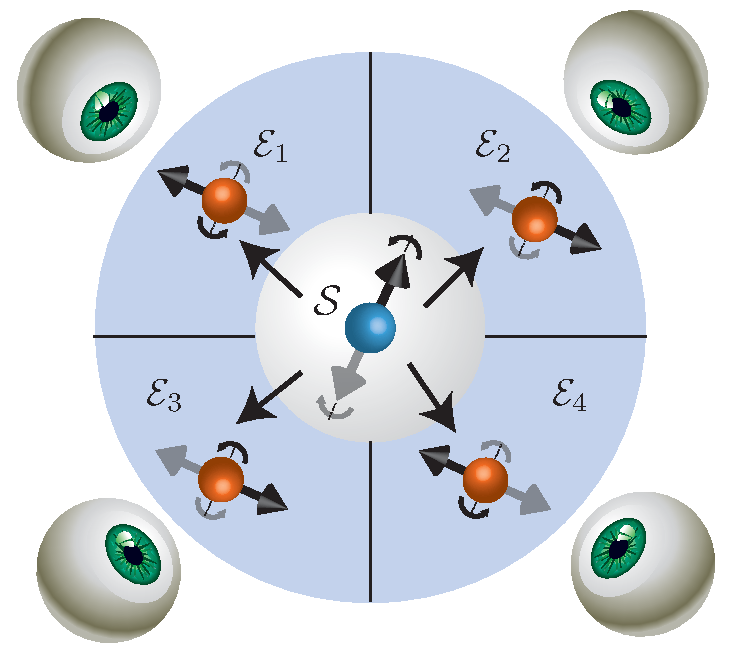
\psfig{file=figure/fig1.pdf, width=0.8\linewidth}}
\caption{The nuclear spin environment as a quantum communication channel. A central electronic spin -- the system $\S$ -- is surrounded by multiple nuclear spins $\E_k$ comprising the environment $\E$. The environment spins are effectively isolated from each other due to their weak spin-spin interaction. The environment decoheres the system and, in the process, each of its components is rotated into a new state (black and grey arrows) conditional on the central spin state. Multiple observers (eyes) can access different environment spins and thus independently deduce the state of the system.}
\label{fig:1}
\end{figure}

We will focus on the single electron spin in an NV center~\cite{DOHERTY20131,PSSA:PSSA200671403}, Fig.~\ref{fig:2}a, embedded in a room-temperature diamond environment that carries nuclear $^{13}$C spins (with the natural abundance of 1.1 \%). Such a platform - a central electron spin coupled to nuclear ancilla spins - has also been studied in previous experiments in different contexts \cite{Taminiau14,Hirose16,Zaiser16}. In the secular approximation~\cite{Childress281}, the Hamiltonian is 
\begin{equation}
\H = 2\pi S_z\sum_k A^k_\parallel I^k_z ,
\label{eq:H0}
\end{equation}
where $S_z = \proj{\up}{\up}$ is a shifted $z$-operator for the electron spin and $I^k_z$ is the corresponding spin-1/2 operator for the nuclear spin $k$. This is of the pure decoherence form, where environment components interact with the system and do not interact with each other~\cite{Zwolak14,zwolak16,Riedel12-1}. The eigenstates of $S_z$ give the so-called pointer states of the system~\cite{Zurek81-1}, the states that are not perturbed by the environment but for which superpositions are decohered. For an initial state where the electron spin is in a ``weird'' quantum superposition, $\ket{+}=\ket{\up}+\ket{\down}$, and in a product state with the environment spins (individually in an initialized state $\ket{\phi_k}$), 
\begin{equation}
\ket{\psi(0)} = \ket{+}_\S \otimes \left[ \bigotimes_k \ket{\phi_k} \right],
\label{eq:Psi0}
\end{equation}
the state after evolving for a time $t$ is
\begin{equation}
\ket{\psi(t)} = \ket{\up}_\S \otimes \left[ \bigotimes_k \ket{\phi_{k|\up}} \right] + \ket{\down}_S \otimes \left[ \bigotimes_k \ket{\phi_{k|\down}} \right].
\label{eq:GHZ}
\end{equation}
The superposition in the system has ``branched out'' into the environment, creating correlations with the nuclear spins via conditional rotations into the states $\ket{\phi_{k|\hat{s}}}$ with $\hat{s}=\up,\down$ the pointer states of the system (the $m_s =0$ and $-1$ states of the NV center, respectively, see Fig.~\ref{fig:2}a). 

When $\ket{\phi_k} = \ket{+}$, $A^k_\parallel=A_\parallel$, and $t=1/2A_\parallel$, the state in Eq.~\eqref{eq:GHZ} is a GHZ state (but with potentially many more than three qubits), where each environment spin holds a perfect record of the pointer state, i.e., the conditional states $\ket{\phi_{k|\up}}$ and $\ket{\phi_{k|\down}}$ are orthogonal. Under more general conditions, the state is GHZ-like and each spin only holds a partial record of the system's state. In either case, it carries redundant information which can be quantified by the quantum mutual information between the system $\S$ and a fragment $\F$ of the environment, 
\begin{equation} \label{eq:MI}
\MI = \ES + \EF - \ESF ,
\end{equation}
where $H_\A=-\tr \rho_\A \log_2 \rho_A$ is the von Neumann entropy of subsystem $\A$. This decomposes into classical and quantum components~\cite{Zwolak13-1}, 
\begin{equation} \label{eq:QC}
\MI = \Hol + \QD ,
\end{equation}
with
\begin{equation}
\Hol = \EF - \sum_{s} p_s \CEF(t)
\end{equation}
giving the Holevo quantity -- an upper bound on the classical information about observable $\Pi_{\S}$ on $\S$ communicated by $\F$ -- and $\QD$ giving the quantum discord~\cite{Zurek00-1,Ollivier02-1,Henderson01-1}. The quantity $\CEF$ is the entropy of $\F$ conditioned on outcome $s$ in $\S$ (with probability $p_s$). In principle, one can examine the information about any observable of $\S$, but under decoherence it is information about the pointer states of $\S$, $\PO$ ($S_z$ in our case), that is imprinted on $\F$~\cite{Ollivier04-1,Zwolak13-1}. In what follows, we will determine $\HolpIL$ in both natural and artificial settings. Since we are ultimately concerned with the emergence of classical objectivity in natural settings, the quantum information, $\QDpIL$, is difficult to access due to the interactions with many environment spins inaccessible to the measurement, as well as the complexity of the measurement itself. We thus focus only on $\HolpIL$ and will discuss possibilities for obtaining $\QDpIL$ afterward.

In the case of a perfect GHZ state, the Holevo information is 1 bit for any fragment of the environment: If there are, e.g., several observers which each intercept one spin from the environment, they can all independently determine the (pointer) state of the system. This is the notion of redundancy, that there are (in this ideal case) $\Es$ copies of the information about the system in the environment of size $\Es$. Departing from ideality, the redundancy, $R_\delta$, will be $\Es/\Fd$ where $\Fd$ is the size of the typical fragment required to get to obtain
\begin{equation} \label{eq:Red}
\avg{\HolpIL} \ge (1-\delta) \HPB .
\end{equation}
That is, the fragment size, on average, to get more than $\HPB$ of the missing information about $\S$. The quantity $\delta$ is the information deficit -- the finite precision one has to pay for lack of ideality. 

\begin{figure*}
\centerline{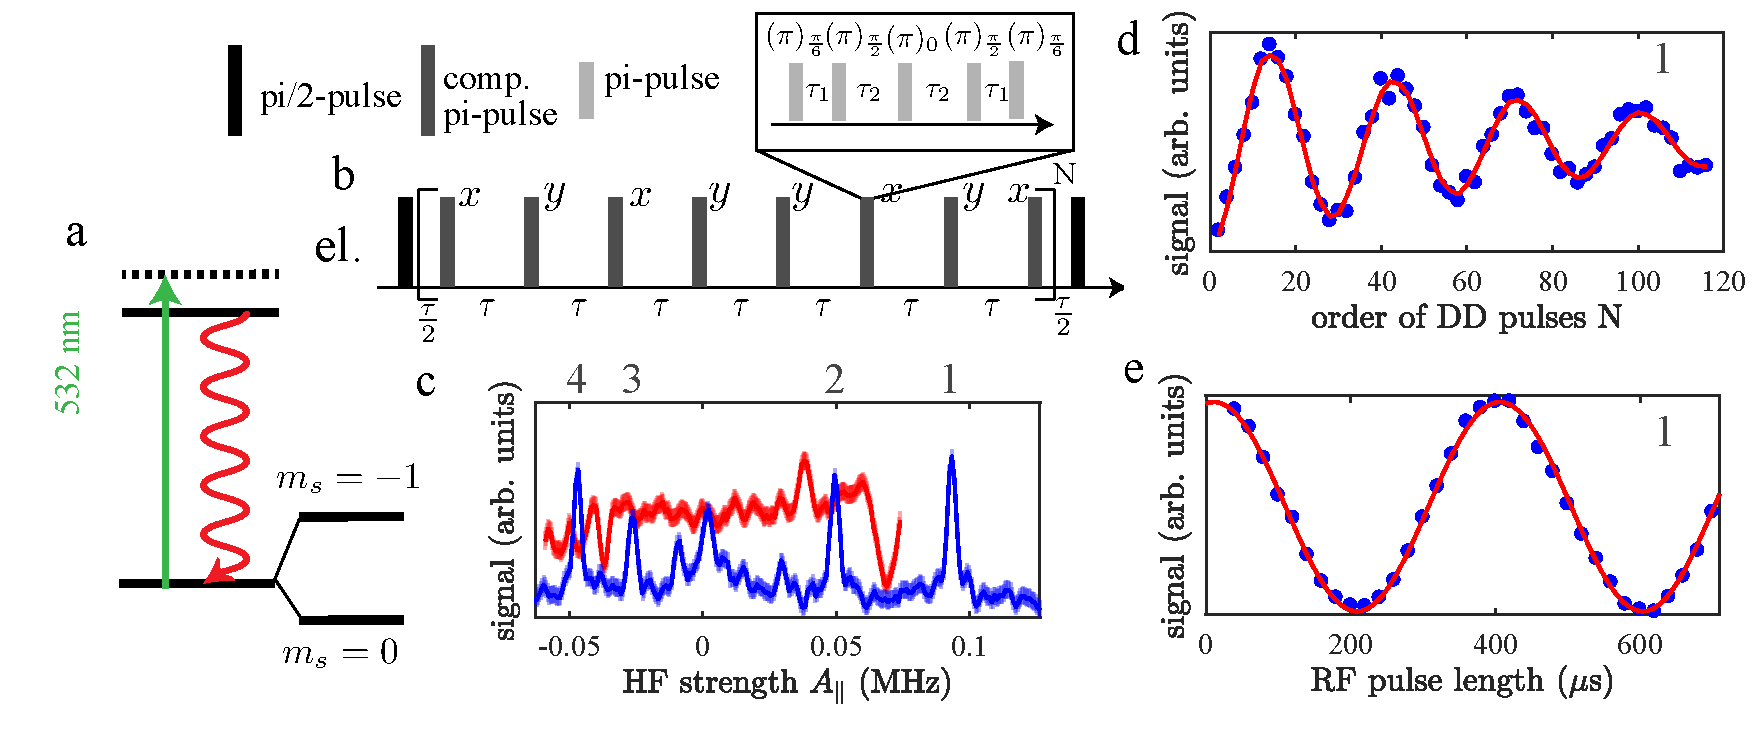
\psfig{file=figure/fig2.pdf, width=0.8\linewidth}}
\caption{Experimental control of the nuclear-electronic spin system. (a) Energy level diagram of the electronic spin of an NV center. The orbital configuration can be optically excited with a green laser light and the passage through the excited state is manifest by red fluorescence. Each orbital state carries a spin triplet ($S=1$) manifold. Spin-dependent non-radiative decay can be used for optical spin detection and efficient spin initialization of the ground state. In this work we focus on the two-level-system specified by the ground state spin sublevels $\ket{m_s=0} \equiv \ket{\up}$ and $\ket{m_s=-1} \equiv \ket{\down}$. (b) The adaptive XY8$^N$  sequence. The DD is a train of composite $\pi$-pulses with an interpulse spacing of $\tau$ and an alternating phase for robustness. Each $\pi$-pulse is a symmetric sequence of five microwave $\pi$-pulses (inset) with different pulse phases also to achieve robustness against single pulse imperfections. By tuning $\tau$ to the Larmor precession of nuclear carbon spins, resonant electron-nuclear spin interaction is achieved. Additional time evolution ($\tau_1,\tau_2$) incorporated in the composite $\pi$-pulses is used to control the strength of the resonant interaction. (c) Measured spectrum (blue) when the interpulse spacing $\tau = 1/(\omega_L+A_{\parallel}/2)$ of an AXY$^{16}$ sequence varies, where $\omega_L$ specifies the bare Larmor frequency of nuclear carbon spins determined by the external, applied magnetic field (here, $\approx 470$ kHz). The $x$-axis is already converted to the parallel component of the hyperfine (HF) interaction. The natural electron-nuclear spin interaction strength is reduced by the incorporation of an additional free evolution during robust pulses. Compared to a standard XY8$^{16}$ method (red), four isolated carbon spins $k=1,\ldots,4$ are visible (shaded blue) under the AXY8$^{16}$ pulse sequence. The solid lines are smoothed data and the light blue/red shaded regions represent one standard deviation. (d) NV spin mediated Rabi oscillations of a single nuclear spin. The interpulse spacing $\tau$ is tuned to the Larmor period of carbon spin 1 and the order $N$ of the DD sequence is increased. The red curve is the result of a simulation, when the measured hyperfine values (see the Supplemental Information) are taken into account. (e) Rabi oscillation of nuclear spin 1 driven by an RF field. NV mediated nuclear gates are used for initialization and readout of the nuclear spin. The solid curve is a cosine fit corresponding to a sum of squares error (SSE) of $2.4\cdot10^{-4}$. Errors are smaller than the data points in (d,e).}
\label{fig:2}
\end{figure*}

It is clear that to observe this process in the laboratory, one either has to perform full quantum state tomography or, to see that there is redundant information, address the individual nuclear spins. State-of-the-art technology uses Dynamical Decoupling (DD) to address issues such as these. However, selectivity in a spectrally dense environment is still a difficult task. Here, we implement a novel DD protocol, theoretically proposed in Refs.~\cite{Cas2015,Cas17}, to both identify the spin environment and to control individual parts of it. Like well-established DD sequences such as CPMG~\cite{MAUDSLEY1986488} or XY8~\cite{gull90}, the protocol employs repetitive central spin flips via a microwave (MW) drive, where the inter pulse spacing determines the frequency of the control window. However, the new protocol, the adaptive XY8 (AXY8) sequence, establishes a robust control of individual nuclear spins mediated by the central electron spin by arbitrarily shaping the DD control-filter, see Fig.~\ref{fig:2}b. This refocuses undesired noise, allowing for the identification and control of individual nuclear spins. 

More specifically, control of the filter design is supplied by replacing each single spin flip by a train of five pulses, see the inset of Fig.~\ref{fig:2}b. An alternating rotation axis (phase) of the MW pulses permits a robust operation in the presence of pulse errors. Time evolution during the pulse train models an arbitrary filter response, where the evolution times $\tau_1$ and $\tau_2$ are numerically calculated with a specific filter function, see the Methods. In general, the process is modeled by the effective Hamiltonian~\cite{Cas2015}
\begin{equation}
H^k = 2\pi f_{DD} \left(S_z -\frac{1}{2}\right) I^k_x,
\label{eq:EM1}
\end{equation}
when the interpulse spacing $\tau$ matches the corresponding Larmor frequency of nuclear spin $k$. $I_x^k$ is the corresponding nuclear spin-$1/2$ operator in $x$-direction. 

The effective interaction strength $f_{DD}$ is mediated by the perpendicular HF coupling $A_\perp$, which is here determined by the magnetic dipole-dipole interaction. Instead of a constant interaction strength, determined by $A_\perp$, a weaker effective strength can be modeled without the necessity of using high harmonics~\cite{Childress281,Tam14}, which are more vulnerable to pulse error, to achieve individual nuclear spin addressing. An AXY spectrum of the nuclear spin environment is shown in Fig.~\ref{fig:2}c (blue curve). Due to electron-nuclear spin entanglement governed by Eq.~\eqref{eq:EM1}, four nuclear spin and additional, more weakly coupled ones can be identified by their different parallel HF interaction strength, when the interpulse spacing $\tau$ varies. The effective coupling strength was here reduced by about a factor of five compared to the natural strength determined by the register geometry. The result of the typical, non-adaptive XY8 sequence (red curve) doesn't show the features. The natural interaction strength is too strong, and therefore the resonances too broad to identify individual spins. The rising and falling of quantum correlations between the electronic spin and a nuclear spin is shown in Fig.~\ref{fig:2}d, when the repetition $N$ of the pulse sequence is increased, while the pulse spacing is kept constant.

For further control, nuclear spin initialization and individual measurement via optical readout of the NV electronic spin is necessary. We achieve both by using the entangling gate (explained above), in combination with an asymmetric version~\cite{Souza4748} of it, to implement an iSwap gate ($e^{i\frac{\pi}{2}\sigma_xI_x}e^{i\frac{\pi}{2}\sigma_yI_y}$)~\cite{Cas17}. For the strongest coupled nuclear spin, it takes about $50\mu s$ to perform a swap operation, and for the weakest coupled one about $80\mu s$. We implement the entangling gate $R=e^{iH^k\frac{\pi}{2}}$ for each nuclear spin by carefully adjusting the repetition $N$ of the AXY sequence and the interpulse spacing $\tau$. For example, the result in Fig.~\ref{fig:2}e shows Rabi oscillations of nuclear spin one induced by a resonant radio frequency (RF) field. First the electron spin was optically polarized, then polarization was swapped to nuclear spin 1 with additional reinitialization of electron spin, application of the RF pulse follows and nuclear spin information is optically read out after a second iSwap gate. A typical gate fidelity of an iSwap gate is on the order of $0.8$ and is mainly limited by the electron coherence time of about 0.7 ms. Specific HF coupling values of the four nuclear spin system can be found in the Supplemental Information (SI). Using this approach, we first show the controlled creation and the characterization of a redundant state in a three nuclear spin system coupled to the central electronic spin. We then select the four strongest coupled nuclear spins and explore the rising and falling of redundancy in time mediated by the natural HF interaction.

\begin{figure}
\centerline{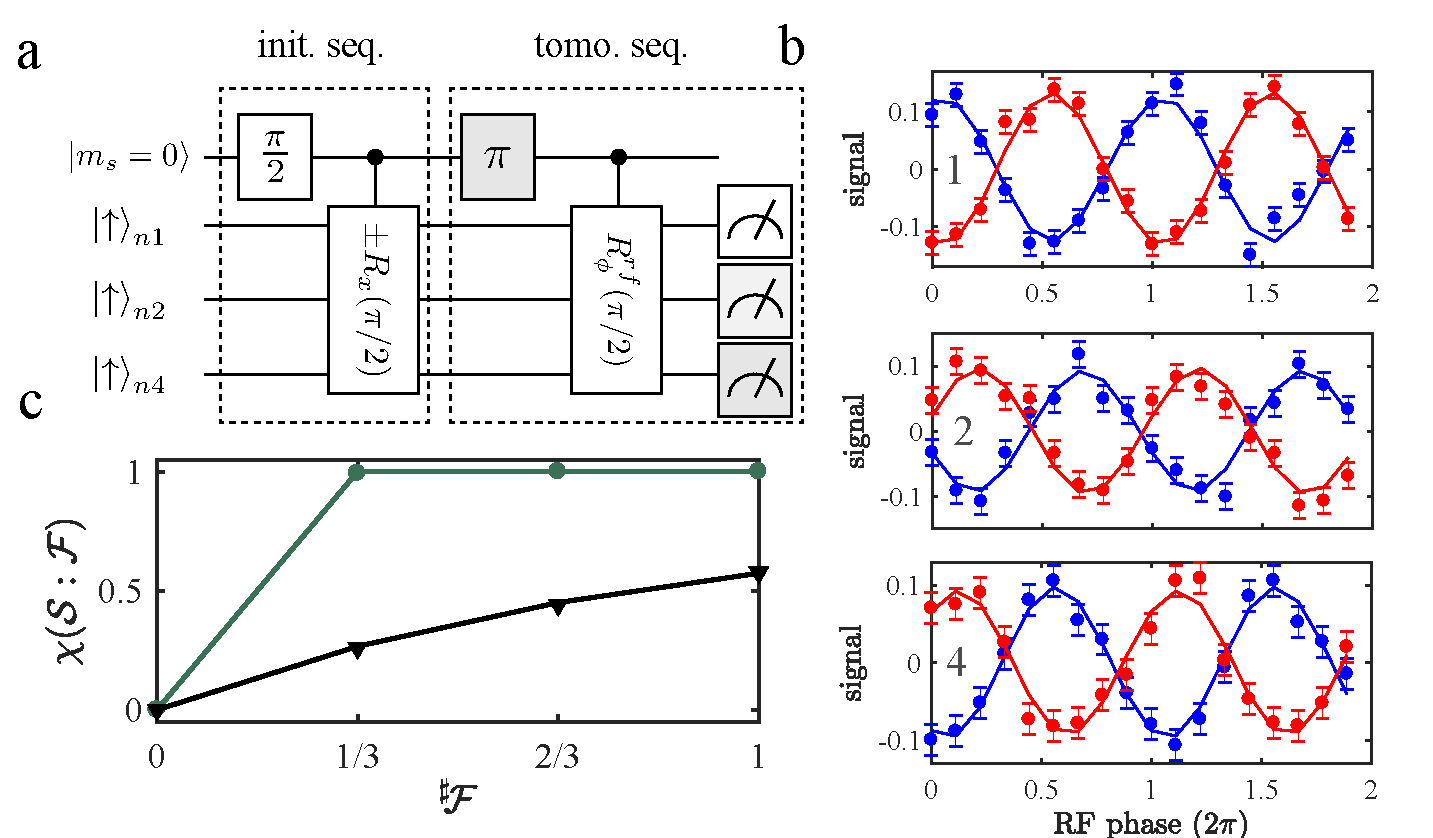
\psfig{file=figure/fig3.pdf, width=1.1\linewidth}}
\caption{Storing the central spin state redundantly in a three nuclear spin environment. (a) Protocol for creation and readout of the redundant state. The NV spin is first initialized and its polarization swapped to each individual nuclear spin by a repetitive process (not shown). An electronic superposition is then created by a $\frac{\pi}{2}$-pulse. Electronic-nuclear spin entanglement is created by a $\frac{\pi}{2}$ nuclear rotation in a direction conditional on the electronic spin state (see text). Single nuclear spin tomography in the electronic subspace $\ket{m_s=-1}$ is performed by a conditional $\frac{\pi}{2}$-pulse mediated by weak, resonant RF pulses applied to the three nuclear spins. In addition, multiple measurements are performed with a different RF pulse phase $\phi$ to determine the phase of the nuclear spin superposition. An optional $\pi$-pulse in front of the last RF pulses can be applied for nuclear spin tomography in the electronic $\ket{m_s=0}$ subspace. The state of a single nuclear spin is in the end swapped to the NV spin and an optical readout follows. In a single sequence run, a nuclear spin is readout in one of the electronic subspaces. (b) Measurement results corresponding to the sequence shown in (a). The normalized NV fluorescence for each nuclear spin $(1,2,4)$ is presented. Tomography in the $\ket{m_s=0}$ ($\ket{m_s=-1}$) subspace is indicated in blue (red). Solid curves are results of a simulation (see Methods). Error bars represent one standard deviation of the measured data points. (c) Holevo information $\HolpIL$ based on the analysis of the data in (b) when different environment fraction sizes $\Fs$ are taken. The black data is corrected for error happening during tomography step (see the Methods) and the dark green data is also corrected for imperfect initial polarization. The solid curves show the results of a simulation considering the entangled state, Eq.~\eqref{eq:GHZ}, with introduced initial polarization imperfections (black) and without (dark green). Errors are smaller than the data points.} 
\label{fig:3}
\end{figure}

The protocol to create a GHZ state is in Fig.~\ref{fig:3}a. For this demonstration, the three strongest coupled nuclear spins are chosen. We polarize the nuclear spins by first polarizing the electron spin via optical pumping and then swapping the electron polarization to each nuclear spin. This is followed by an electronic $\pi/2$-pulse and entanglement is sequentially created by the application of the gate described above. To observe correlations with a single nuclear spin, we utilize a selective RF $\pi/2$-pulse with variable phase $\phi$ ($R^{rf}_\phi$), which only flips the nuclear spin when the NV center is in the $m_s = -1$ state. To have access to the $m_s=0$ state, an optional MW $\pi$-pulse can be applied in front of the RF pulse. The results are shown in Fig.~\ref{fig:3}b for each nuclear spin. By varying the phase of the RF pulse, oscillations occur. For all nuclear spins we observe a $\pi$-phase shift between the data observed in the $m_s = 0$ (in blue) and $m_s = -1$ (in red) state, which indicates the orthogonal preparation of the state shown in Eq.~\eqref{eq:GHZ}. The phase shift between signals of different nuclear spins is due to a different HF tensor with respect to the laboratory frame, defined by the RF-field axis~\cite{Laraoui15}. Here we focus mainly on classical correlations, but the results of an echo kind of sequence shows also the presence of quantum correlations in form of multiple quantum coherences~\cite{Baum85,Gaerttner17}, see the SI.  

Figure~\ref{fig:3}c presents the Holevo information versus the fraction of nuclear spins in the fragment. In black we show the analyzed data, when error happening during the tomography sequence are corrected and in dark green the results when also error due to imperfect initial nuclear spin polarization is corrected (details are in the Methods). The typical degree of polarization is on the order of $(75\pm 5) \%$ for each nuclear spin and the fidelity of for creating the GHZ state is about $40$ \% (see the SI). Focusing on the data set shown in green, as soon as just one spin from the environment is intercepted, the Holevo information is already 1 bit. That is, access to a single environment spin already gives the pointer state of the system. Interception of further spins does not increase the Holevo information but only confirms the information from the first. This plateau -- the classical plateau -- signifies the appearance of redundant information. When error due to imperfect initial polarization are not corrected (black data), only the initial rise to the plateau is seen. Due to a non-zero initial entropy, the amount of information a single nuclear spin can store decreases and even when all environmental spins are taken into account, only about half a bit of central spin information can be intercepted. In general this is not true when a larger spin environment is considered~\cite{Zwolak09,Zwolak10-1}. 

\begin{figure*}
\centerline{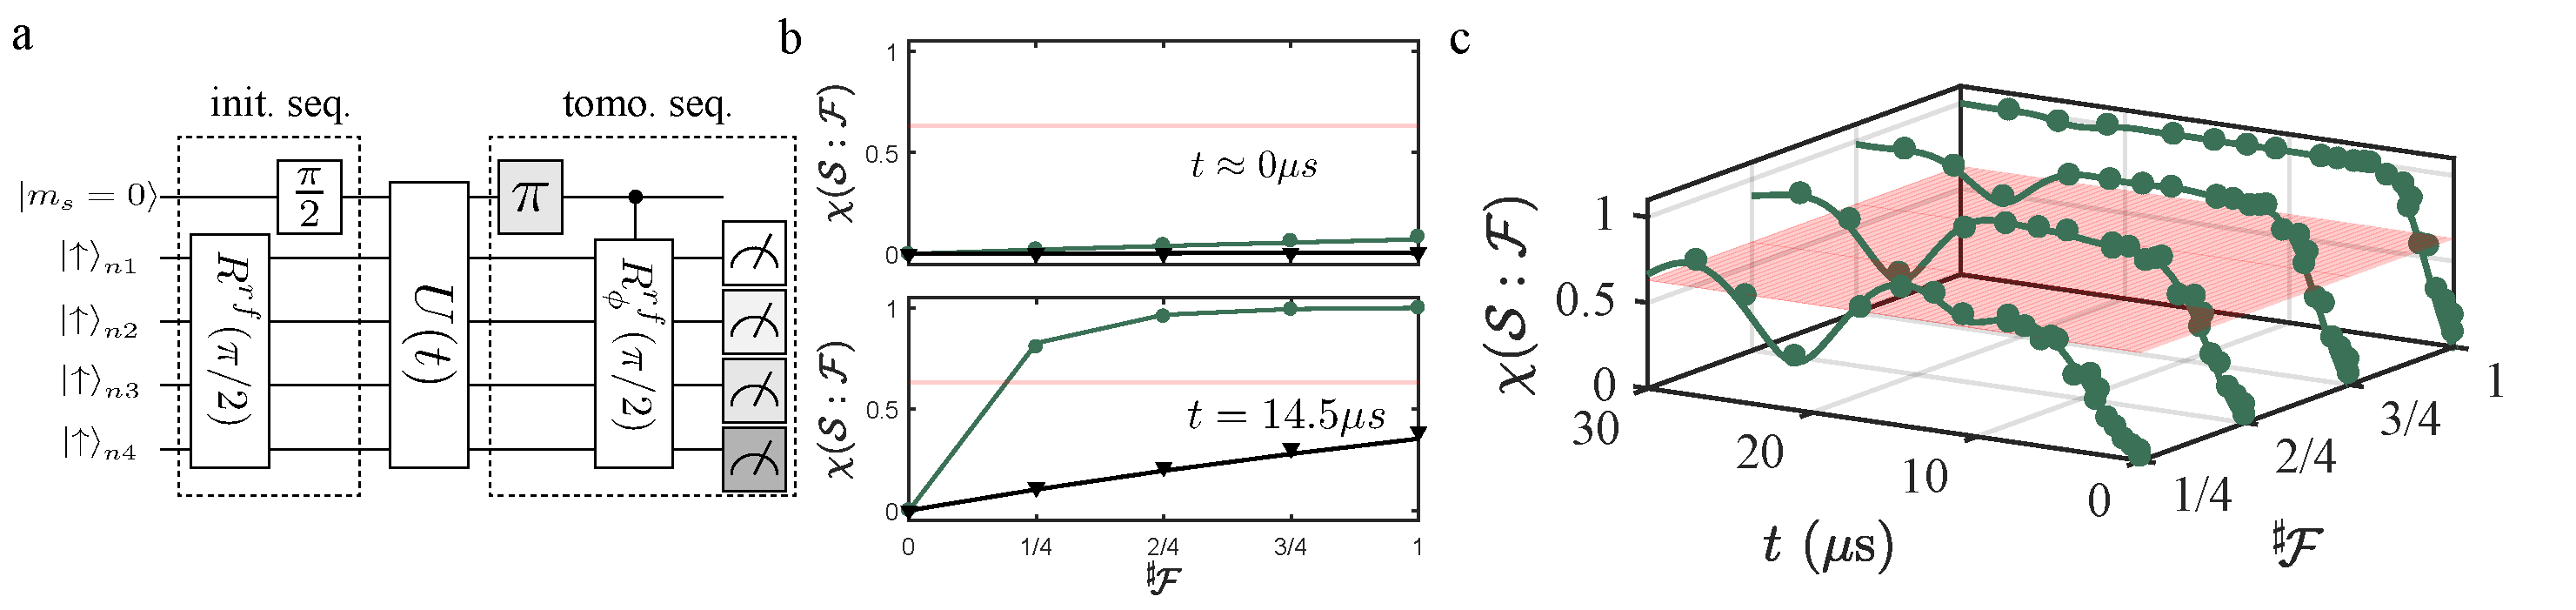
\psfig{file=figure/fig4.pdf, width=1\linewidth}}
\caption{The emergence of redundancy for an NV center being naturally decohered by its environment. (a) Compared with Fig.~\ref{fig:3}, the measurement protocol changes the initialization sequence and adds a free evolution, $U$, with a duration of $t$. After polarization, two $\frac{\pi}{2}$-pulses transform the product state into a product state of $\ket{+}$ states. These then evolve under the direct HF interaction between the NV center and nuclear spins. The tomography sequence is the same as in Fig.~\ref{fig:3}. (b) Holevo information versus fraction size for a few different times. For small times, there are no correlations between $\S$ and $\E$. However, as decoherence occurs, information is transferred into $\E$ resulting in the formation of a {\em classical plateau}. The plateau signifies the appearance of redundant information. When the data is not normalized to the initial degree of polarization (black), only the initial rise of information is seen. (c) Holevo information, $\HolpIL$, versus the environment fragment size $\Fs$ and free evolution time $t$. For small fractions one can see the initial rise in information with time followed by oscillations. This is due to information flowing into the fragment of the environment and then back into the system (i.e., more strongly interacting environment spins will first gain information and then transfer it back to $\S$). For larger fractions, however, one sees just a rise and a plateau with time. This is due to different interaction strengths with the environment spins, overall tending to force the information flow one way. The solid curves in (b) and (c) show the result of  simulations with and without imperfect initial polarization. The dynamics in simulation are governed by the Hamiltonian $H_0$, Eq.~\eqref{eq:H0}. The semi-transparent red lines in (b) and the plane in (c) indicate an information deficit of $1/e$, i.e., $I = (1-1/e) H_\S$. Errors are smaller than the data points.}
\label{fig:4}
\end{figure*}

In the above, redundancy is created artificially via the construction of a GHZ state, which was also achieved recently with photonic simulators~\cite{Ciampini18-1,Chen18-1}. In addition, previous work on the field of quantum non-demolition (QND)  measurements \cite{Nogues99,Gleyzes07,Lupascu07,Neumann542} were also able to create highly redundant states by consecutive two-body scattering. However, in our everyday world, redundancy appears as a consequence of natural interactions between an $\S$ and $\E$ initially out of equilibrium. To observe this in NV centers, we have to allow the system to evolve in the presence of the HF interaction rather than the artificially applied DD sequences. The experimental protocol is shown in Fig.~\ref{fig:4}a. We first initialize the system into the out-of-equilibrium product state, Eq.~\eqref{eq:Psi0}, with $\ket{\phi_k}=\ket{+}$. This is followed by the free evolution of $\S\E$ of duration $t$ according to the HF Hamiltonian, Eq.~\eqref{eq:H0}. To determine the classical correlations of fragments, $\F$, of the environment with $\S$, the same tomography sequence as above is employed.

Figure~\ref{fig:4}b shows the Holevo information versus fraction size for a few evolution times and Fig.~\ref{fig:4}c shows the full data. The dark green data show again the results when error due to imperfect polarization are normalized with respect to the observed initial polarization of the environmental fragments. At short times, there is essentially no information in fragments or even the whole environment, as initially the $\S\E$ state is a product state. As time develops, however, information is rapidly transferred into the environment. At a time of 14.5 $\mu s$ even a single nuclear spin captures nearly complete information, to within an information deficit of $1/e$ bits. In other words, all the four most strongly coupled nuclear spins have nearly a complete record of the system's pointer state. This redundancy is signified by the presence of a plateau in the Holevo information versus fragment size. We note also that the timescale of information rising (on the order of several $\mu$s) is in good agreement with the NV spin coherence time measured by a Ramsey experiment, see the SI. With increasing time, though, small fragments will see information flow back into the system. This is due to the fact that for individual spins the conditional states first get rotated away from each other and then back towards each other. For sufficiently large number of spins with random interaction strengths, even this information flow into a single spin will be one way on average. For larger fragment sizes, the information tends more and more to be one way, although there will still be periods of recurrence for long enough waiting times. When the experimental data are not normalized with respect to the initial degree of polarization (black data), redundancy is again suppressed due to the lower -- but nonzero except for cases of measure zero~\cite{Zwolak14,zwolak16} -- information capacity of the ``hazy'' environmental fragments~\cite{Zwolak09,Zwolak10-1}. The absolute amount of redundancy is therefore different when normalization with respect to the limited initial nuclear spin polarization and correction of error coming from readout are taken into account compared to only the faulty readout. It is important to note that normalization takes only faulty (and well characterized) processes before and after the buildup of nuclear-electron spin correlations into account. Comparing our results with the results of simulations shows that error during nuclear-electron spin interaction are negligible.

We have focused on the emergence of redundancy under decoherence. This study, though, gives a path forward to see also the banishment of quantum information -- the fact that there was initially a superposition that gets transformed into global quantum correlations. This global coherence leaves a signature in the quantum mutual information ($\QDpIL$, the counterpart to $\HolpIL$ in Eq.~\eqref{eq:QC}) in the form of an ``uptick'' when the whole (or nearly whole) environment is intercepted~\cite{Zwolak13-1}. This can be observed artificially in, e.g., isolated photonic simulators~\cite{Ciampini18-1,Chen18-1}. Within natural settings, though, interactions with inaccessible environment components, as well as imperfect readout/initialization of the accessible environment components, make observing the uptick very challenging. Indeed, the inaccessibility of the uptick due to the interactions with many environment components is what makes our everyday world classical~\cite{Zwolak13-1}. Thus, it is no surprise that it is difficult to measure in naturally decohering systems. Further refinement of the DD technique and samples, together with low temperature measurements, may make this uptick accessible. This will motivate future experiments in NV centers embedded in moderately $^{13}$C enriched diamond (see the SI) to observe large amounts of redundancy.

To conclude, these results give the first laboratory demonstration of quantum Darwinism in action in a natural environment. This required implementing a novel DD protocol to observe. The process by which nuclear spin decoherence of NV centers gives rise to classical objectivity is the same as that occurs due to photons in our macroscopic world. In both cases, the weird quantum superpositions are embedded in a much larger environment, initially out of equilibrium. Interactions with the environment select certain preferred states, decohering their superpositions and proliferating accessible information about them into the world, relegating non-redundant quantum correlations to the dustbin of inaccessibility. \\

\section*{\label{sec:Methods} Methods}

\subsection*{\label{sample}Experimental Setup and Control}

The diamond sample (IIa) is grown via chemical vapor deposition. The isotopic composition is $98.9$ \% $^{12}C$. The concentration of carbon isotope nuclear spins ($1.1$ \% $^{13}$C) gives a significant probability to find multiple weakly coupled $^{13}$C in the frozen core of a native (un-implanted) NV center, the ones we employ for qubits.

For optical manipulation and detection of single NV centers in bulk diamond, we use a home-built confocal microscope and, for initialization and readout of the NV ground state spin, green laser excitation ($532$ nm). An avalanche photodiode detects the corresponding fluorescence and a permanent magnet gives the static field ($\approx440$ G). We drive the electronic (NV) and nuclear ($^{13}$C) spin transitions via MW and RF fields via a thin copper wire close to the NV center and an arbitrary-wave form generator. The MW/RF phase gives the rotation axis of a pulse. We insert a $\frac{\pi}{2}$ phase-shift to get rotations around the $y$-axis. For manipulation, the typical Rabi frequencies are $40$ MHz for the electron spin rotations and $5kHz$ for nuclear spin rotations.

The DD sequence proposed in Ref.~\cite{Cas2015} provides control. Adjusting the timing $(\tau_1,\tau_2)$ and interpulse spacing $\tau$ can give an arbitrary filter-function for the DD sequence. We focus on the first harmonic and set the other contributions up to $4^{th}$ order to zero. The strength of the filter-function is set by the filter coefficients  $f_1=f_{DD},f_2=0,f_3=0,f_4=0$ and we solve the equations (see Ref.~\cite{Cas2015})
\begin{equation}
f_n = -\frac{4}{n \pi} \sum_{i=1}^{5} (-1)^i \sin(n \theta_i)
\end{equation}
for $n=1-4$ numerically to get the corresponding pair of times 
\begin{align}
\tau_1 &= \frac{\theta_1}{2\pi}\cdot\frac{1}{\omega_{DD}}\\
\tau_2 &= \frac{\theta_1}{2\pi}\cdot\left(\theta_2-\theta_1\right)\cdot\frac{1}{\omega_{DD}}.  
\end{align}
The frequency $\omega_{DD}=\frac{1}{\tau}$ is the center of the control filter and $\theta_5 = \theta_2 + \theta_4 -(\theta_1 + \theta_3) + \pi/2$. Any effective coupling $f_{DD}\in \frac{A_\perp}{2\pi}\left(-8\cos(\frac{\pi}{9})+4,8\cos(\frac{\pi}{9})-4\right)$ is possible, where $A_\perp$ is the perpendicular HF coupling strength of an individual nuclear spin. In the SI, we show the coherent interaction between the electron and nuclear spins for different strengths and other parameters.

\subsection*{\label{sec:analysis}Analysis}

The Holevo information requires the diagonal (in the $\PB$ basis of the system) component of the $\S\E$ density matrix. We thus can take the density matrix to be of the form $\rho_{\S\E}= p_{\up} \proj{\up}{\up} \otimes \rho_{\E\left|\up\right.} + p_{\down} \proj{\down}{\down} \otimes \rho_{\E\left|\down\right.}$, where the off-diagonal components in $\PB$ are not present (e.g., $\proj{\up}{\down}$ and $\proj{\down}{\up}$) and $\rho_{\E\left|\hat{s}\right.}=\bigotimes_k \rho_{\E_k\left|\hat{s}\right.}$ are the conditional nuclear density matrices in the corresponding electronic spin (pointer) sublevel $\hat{s}$. We determine the parameters of the nuclear density matrices by fitting the experimental data with simulation (and $p_{\up} = p_{\down} = 1/2$). The Lindbladian for the simulation consists of the coherent HF interaction, Eq.~\eqref{eq:H0}, and a pure dephasing term associated with the HF coupling to additional, weakly coupled nuclear spins and spin flip-flop processes between them. We precisely measure in advance the parallel and perpendicular components (the perpendicular is only important in readout and polarization step) of the HF coupling to the four core spins and the dephasing rate. By performing this fitting, we correct the $\S\E$ density matrix for errors occurring during the tomography process. To correct also the impact of imperfect nuclear spin initialization, the individual nuclear spin density matrices need to take on the form 
\begin{equation}
\rho_{\E_k} = \begin{pmatrix}
\rho_{11} & \rho_{12}/P_k\\
\rho_{21}/P_k & \rho_{22}
\end{pmatrix} ,
\end{equation}
where $P_k$ is the initial degree of nuclear spin polarization (after the swap operations) from the previous analysis step. This normalizes the experimental data to the optical contrast of NV Rabi oscillations. 

\section*{\label{sec:Acknowledgement} Acknowledgement}
We thank Jorge Casanova, Zhenyu Wang, Liam P. McGuinness, and C. Jess Riedel for helpful discussions. This work was supported by the DoE LDRD program at Los Alamos National Laboratory, FQX, ERC, VW Stiftung,  BW Stiftung, DFG and BMBF.

\bibliographystyle{apsrev}
\bibliography{reference}

\end{document}

